%% chapter 4, by Lesley
%\input{header}
%
%\begin{document}
%
%% First page number
%\setcounter{page}{1}
%% PREVIOUS section number
%\setcounter{section}{3}
%% PREVIOUS subsection number
%\setcounter{subsection}{0}
%
%% ***********************************************************************
%\textsc{Learning in Complex Systems \hfill Spring 2015$\;$ \\
%Lecture Notes \hfill  Shie Mannor, based on notes by Nahum Shimkin}
%\vspace{-18pt}
%\par
%\hrulefill
%% ***********************************************************************
%
%% {\large

%\section{Reinforcement Learning -- Basic Algorithms}

\section{Introduction}

RL methods essentially deal with the solution of (optimal) control problems using
on-line measurements.
We consider an agent who interacts with a dynamic environment,
according to the following diagram:
\bigskip

\begin{figure}[ht]
\begin{center}
\setlength{\unitlength}{3947sp}%
%
\begingroup\makeatletter\ifx\SetFigFont\undefined%
\gdef\SetFigFont#1#2#3#4#5{%
  \reset@font\fontsize{#1}{#2pt}%
  \fontfamily{#3}\fontseries{#4}\fontshape{#5}%
  \selectfont}%
\fi\endgroup%
\begin{picture}(4824,1824)(1189,-2173)
\thinlines
{\put(1201,-2161){\framebox(1275,1800){}}
}%
{\put(4726,-2161){\framebox(1275,1800){}}
}%
{\put(2476,-886){\makebox(1.6667,11.6667){\SetFigFont{5}{6}{\rmdefault}{\mddefault}{\updefault}.}}
}%
{\put(4726,-1786){\vector(-1, 0){2250}}
}%
{\put(4726,-1411){\vector(-1, 0){2250}}
}%
{\put(2476,-736){\vector( 1, 0){2250}}
}%
\put(1426,-1336){\makebox(0,0)[lb]{\smash{\SetFigFont{12}{14.4}{\rmdefault}{\mddefault}{\updefault}{Agent}%
}}}
\put(4851,-1411){\makebox(0,0)[lb]{\smash{\SetFigFont{12}{14.4}{\rmdefault}{\mddefault}{\updefault}{Environment}%
}}}
\put(3226,-586){\makebox(0,0)[lb]{\smash{\SetFigFont{12}{14.4}{\rmdefault}{\mddefault}{\updefault}{Action}%
}}}
\put(3301,-1261){\makebox(0,0)[lb]{\smash{\SetFigFont{12}{14.4}{\rmdefault}{\mddefault}{\updefault}{State}%
}}}
\put(3301,-1711){\makebox(0,0)[lb]{\smash{\SetFigFont{12}{14.4}{\rmdefault}{\mddefault}{\updefault}{Reward}%
}}}
\end{picture}
\end{center}
 %  \epsfig{figure=rhocorhocalcounterexample.eps,width=7.0cm,height=5.95cm}}
% \caption{  }
\label{fig4_1}
\end{figure}
\bigskip

Our agent usually has only partial knowledge of its environment, and therefore
will use some form of {\em learning} scheme, based on the observed signals.
To start with, the agent needs to use some parametric {\em model} of the environment.
We shall use the model of a stationary MDP, with given state space and actions space.
However, the state transition matrix $P=(p(s'|s,a))$ and the immediate reward function
$r=(r(s,a,s'))$ may not be given.
We shall further assume that the observed signal is indeed the state of the
dynamic process (fully observed MDP), and that the reward signal is the immediate
reward $r_t$, with mean $r(s_t,a_t)$.
% (for simplicity we shall use the simplified reward function $r(s,a)$ from here on).

It should be realized that this is an {\em idealized} model of the environment,
which is used by the agent for decision making. In reality, the environment
may be non-stationary, the actual state may not be fully observed (or not even be
well defined), the state and action spaces may be discretized, and the environment
may contain other (possibly learning) decision makers who are not stationary.
Good learning schemes should be designed with an eye towards robustness to these modelling
approximations.


\paragraph{Learning Approaches:} The main approaches for learning in this context can
be classified as follows:
\begin{itemize}
\item Indirect Learning: Estimate an explicit model of the environment
($\hat{P}$ and $\hat{r}$ in our case),
and compute an optimal policy for the estimated model (``Certainty Equivalence" and R-MAX that we saw a few lectures ago).
\item Direct Learning: The optimal control policy is learned without first learning
an explicit model. Such schemes include:

a. Search in policy space: Genetic Algorithms, Policy Gradient....

b.  Value-function based learning, related to Dynamic Programming principles:
 Temporal Difference (TD) learning, $Q$-learning, etc.
\end{itemize}
RL initially referred to the latter (value-based) methods, although
today the name applies more broadly. Our focus in the chapter will be
on this class of algorithms.


Within the class of value-function based schemes, we can distinguish two
major classes of RL methods.

\begin{enumerate}
  \item \textbf{Policy-Iteration based schemes (``actor-critic" learning):}
\begin{center}
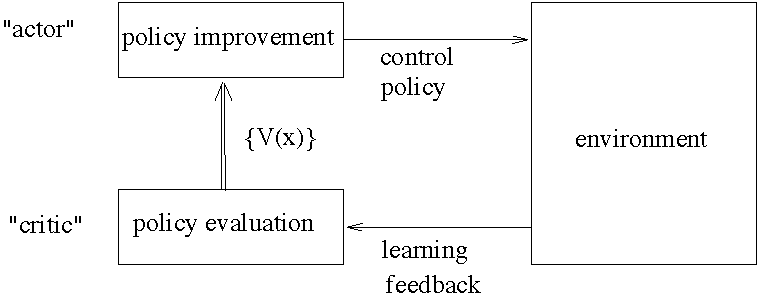
\includegraphics{FIGS/ACRL.pdf}
\end{center}
The ``policy evaluation'' block essentially computes the value function $V^\pi$ under
the current policy (assuming a fixed, stationary policy).
Methods for policy evaluation include:
\begin{enumerate}
  \item ``{Monte Carlo}'' policy evaluation.
  \item Temporal Difference methods - {TD($\la$)}, SARSA, etc.
\end{enumerate}
The ``actor'' block performs some form of policy improvement, based on the
policy iteration idea:
$\bar{\pi} \in \argmax \{r+P^\pi V^\pi\}$.
In addition, it is responsible for implementing some ``exploration'' process.

\item \textbf{Value-Iteration based Schemes:}
These schemes are based on some on-line version of the value-iteration recursions:
$V_{t+1}^* = \max_\pi [r^{\pi}+P^{\pi} V_t^*]$.
The basic learning algorithm in this class is {\em $Q$-learning}.
\end{enumerate}

\section{Example: Deterministic $Q$-Learning}

To demonstrate some key ideas, we start with a simplified learning algorithm
that is suitable for a {\em deterministic} MDP model, namely:
\begin{align*}
& s_{t+1}=f(s_t,a_t) \\
& r_t=r(s_t,a_t)
\end{align*}
We consider the discounted return criterion:
\begin{align*}
V^{\pi}(s) &=\sum_{t=0}^\infty \ga^t r(s_t,a_t)\,,
\quad \text{given } s_0=s, a_t=\pi(s_t)\\
V^*(s) &= \max_\pi V^\pi(s)
\end{align*}
Recall our definition of the $Q$-function (or {\em state-action value function}),
specialized to the present deterministic setting:
$$
Q(s,a)=r(s,a)+\ga V^*(f(s,a))
$$
The optimality equation is then
$$
V^*(s) = \max_a Q(s,a)
$$
or, in terms of $Q$ only:
$$
Q(s,a)=r(s,a)+\ga \max_{a'}Q(f(s,a),a')
$$

Our learning algorithm runs as follows:
\begin{itemize}
\item {\em Initialize:} Set $\hat{Q}(s,a)= Q_0(s,a)$, for all $s$, $a$.
\item At each stage $n=0,1,\dots$:

-- Observe $s_n$, $a_n$, $r_n$, $s_{n+1}$.
% $s\leftarrow s_n$, $a \leftarrow a_n$, $r\leftarrow r_n$, $s'\leftarrow s_{n+1}$.

-- Update $\hat{Q}(s_n,a_n)$:\ \ \
$\hat{Q}(s_n,a_n) := r_n+\ga \max_{a'} \hat{Q}(s_{n+1},a')$
\end{itemize}

We note that this algorithm does not tell us how to choose the actions $a_n$.
The following result is from [Mitchell, Theorem 3.1].

\begin{theorem}[Convergence of $Q$-learning for deterministic MDPs]\ \\
Assume a deterministic MDP model. Let $\hat{Q}_n(s,a)$ denote the estimated
$Q$-function before the $n$-th update.
If each state-action pair is visited \underline{infinitely-often}, then
$\lim_{n\to\infty}\hat{Q}_n(s,a)=Q(s,a)$, for all $(s,a)$.
\end{theorem}

\begin{proof}
Let
$$
\Delta_n \dfn \|\hat{Q}_n-Q\|_\infty = \max_{s,a} |\hat{Q}_n(s,a)-Q(s,a) | \,.
$$
Then at every stage $n$:
\begin{align*}
| \hat{Q}_{n+1}(s_n,a_n)- Q(s_n,a_n)| &= |r_n+\ga\max_{a'} \hat{Q}_n(s_{n+1},a')
- (r_n+\ga\max_{a''} Q(s_{n+1},a'') ) | \\
&= \ga |\max_{a'} \hat{Q}_n(s_{n+1},a') -\max_{a''} {Q}(s_{n+1},a'') | \\
& \le \ga \max_{a'} |\hat{Q}_n(s_{n+1},a') - Q(s_{n+1},a') |
\; \le\;  \ga \Delta_n \,.
\end{align*}
Consider now some interval $[n_1,n_2]$ over which all state-action pairs $(s,a)$
appear at least once. Using the above relation and simple induction, it
follows that $\Delta_{n_2} \le \ga \Delta_{n_1}$. Since $\ga<1$ and since
there is an infinite number of such intervals by assumption, it follows that
$\Delta_n \to 0$.
\end{proof}

\paragraph{Remarks:}
\begin{enumerate}
  \item The algorithm allows the use of an arbitrary policy during learning.
Such an algorithm is called {\em Off-Policy}. In contrast, {\em On-Policy}
algorithms learn the properties of the policy that is actually being applied.
  \item We further note that the ``next-state" $s'=s_{n+1}$ of stage $n$ need not
coincide with the current state $s_{n+1}$ of stage $n+1$. Thus, we may skip
some samples, or even choose $s_n$ at will at each stage. This is a common
feature of off-policy schemes.
  \item A basic requirement in this algorithm is that all state-action pairs will
be sampled "often enough", to ensure that we often use a specific
{\em exploration} algorithm or method. In fact, the speed of convergence
may depend critically on the efficiency of exploration. We shall discuss this
topic in detail further on.
\end{enumerate}

\section{Policy Evaluation: Monte-Carlo Methods}

Policy evaluation algorithms are intended to estimate the value functions
$V^\pi$ or $Q^\pi$ for a given policy $\pi$. Typically these are on-policy
algorithms, and the considered policy is assumed to be stationary (or "almost"
stationary). Policy evaluation is typically used as the ``critic" block of an
actor-critic architecture.

Direct Monte-Carlo methods are the most straight-forward, and are considered
here mainly for comparison with the more elaborate ones. Monte-Carlo methods
are based on the simple idea of averaging a number of random samples of a
random quantity in order to estimate its average.

Let $\pi$ be a fixed stationary policy. Assume we wish to evaluate the
value function $V^\pi$, which is either the discounted return:
$$
V^\pi(s) = E^\pi (\sum_{t=0}^\infty \ga^t r (s_t, a_t) | s_0=s)
$$
or the total return for an SSP (or {\em episodial}) problem:
$$
V^\pi(s) = E^\pi (\sum_{t=0}^T r(s_t, a_t)| s_0=s )
$$
where $T$ is the (stochastic) termination time, or time of arrival to
the terminal state.

Consider first the episodial problem.
Assume that we operate (or simulate) the system with the policy
$\pi$, for which we want to evaluate $V^{\pi}$.
Multiple trials may be performed, starting from arbitrary initial conditions,
and terminating at $T$ (or truncated before).

After visiting state $s$, say at time $t_s$, we add-up the total cost until the
target is reached:
$$
\hat v(s) = \sum_{t=t_s}^T R_t\,.
$$
After $k$ visits to $s$, we have a sequence of total-cost estimates:
$$
\hat v_1 (s) , \cdots, \hat v_k (s)\,.
$$
We can now compute our estimate:
$$
\hat V_k(s) = \frac{1}{k} \sum_{i=1}^k \hat v_i (s)\,.
$$
By repeating these procedure for all states,
we estimate $V^{\pi}(\cdot)$.

\paragraph{State counting options:} Since we perform multiple trials and
each state can be visited several times per trial, there are several options
regarding the visits that will be counted:
\begin{itemize} \negspace
\item[a.]
Compute $\hat V(s)$ only for initial states $(s_0=s)$.
\item[b.]
Compute $\hat V(s)$ each time $s$ is visited.
\item[c.]
Compute $\hat V(s)$ only on first visit of $s$ at each trial.
\end{itemize} \negspace
Method (b) gives the largest number of samples, but
these may be correlated (hence, lead to non-zero bias for finite times).
But in any case, $\hat V_k(s) \to V^{\pi}(s)$ is guaranteed as $k\to\infty$.
Obviously, we still need to guarantee that each state is visited enough
-- this depends on the policy $\pi$ and our choice of initial conditions
for the different trials.

\paragraph{Remarks:}
\begin{enumerate}
  \item The explicit averaging of the $\hat v_k$'s may be replaced by
the iterative computation:
$$
\hat V_k(s) = \hat V_{k-1} (s) + \al_k
\Bigl[\hat v_k (s) - \hat V_{k-1} (s) \Bigr] \,,
$$
with $\al_k=\frac{1}{k}$.  Other choices for $\al_k$ are also common,
e.g.\ $\al_k = \frac{\ga}{k}$, and $\al_k=\eps$
(non-decaying gain, suitable for non-stationary conditions).
  \item For discounted returns, the computation needs to be truncated at some
finite time $T_s$, which can be chosen large enough to guarantee a small
error:
$$
\hat v(s) = \sum_{t=t_s}^{T_s} (\ga)^{t-t_s} R_t\,.
$$
\end{enumerate}

\section{Policy Evaluation: Temporal Difference Methods}

\subsection{The TD(0) Algorithm}\label{ss:TD0}

Consider the total-return (SSP) problem with $\ga=1$.
Recall the fixed-policy Value Iteration procedure of Dynamic Programming:
$$
V_{n+1}(s) = E^{\pi} (r(s,a) + V_n(s') )
           = r(s,\pi(s)) + \sum_{s'} p(s' | s,\pi(s)) V_n(s')\,,\quad \forall s\in S,
$$
or $V_{n+1}  = r^{\pi} + P^{\pi} V_n$, which converges to $V^{\pi}$.

Assume now that $r^{\pi}$ and $P^{\pi}$ are not given.
We wish to devise a ``learning version" of the above policy iteration.

Let us run or simulate the system with policy $\pi$.
Suppose we start with some estimate $\hat V$ of $V^{\pi}$.
At time $n$, we observe $s_n$, $r_n$ and $s_{n+1}$.
We note that $[r_n + \hat V(s_{n+1})]$ is an unbiased
estimate for the right-hand side of the value iteration equation,
in the sense that
$$
E^\pi (r_n + \hat V(s_{n+1}) | s_n) =
r(s_n,\pi(s_n)) + \sum_{s'} p(s' | s_n,\pi(s_n)) V_n(s')
$$
However, this is a {\em noisy} estimate, due to randomness in $r$ and $s'$.
We therefore use it to modify $\hat V$ only slightly, according to:
\begin{align*}
\hat V (s_n) & := (1-\al_n) \hat V(s_n) + \al_n [r_n + \hat V (s_{n+1}) ] \\
& = \hat V(s_n) + \al_n [r_n + \hat V(s_{n+1}) - \hat V(s_n)]
% \underbrace{[r_n + \hat V(s_{n+1}) - \hat V(s_n)]}_{\bydef d_n}
\end{align*}
Here $\al_n$ is the {\em gain} of the algorithm.
If we define now
$$
d_n \dfn r_n + \hat V(s_{n+1}) - \hat V(s_n)
$$
we obtain the update rule:
$$
\hat V (s_n) := \hat V(s_n)+\al_n d_n \,
$$

$d_n$ is called the {\em Temporal Difference}.
The last equation defines the \underline{TD(0) algorithm}.



Note that $\hat V(s_n)$ is updated on basis of $\hat V(s_{n+1})$, which is
itself an estimate.  Thus, TD is a ``bootstrap" method: convergence of
$\hat V$ at each states $s$ is inter-dependent with other states.

\paragraph{Convergence results for TD(0)\quad (preview):}
\begin{enumerate}
\item
If $\al_n \searrow 0 $ at suitable rate ($\al_n \approx 1/$no.~of visits to
$s_n$), and each state is visited i.o., then
$\hat V_n \to V^{\pi}$ w.p. 1.

\item
If $\al_n= \al_0$ (a small positive constant) and each state is visited i.o.,
then $\hat V_n$ will ``eventually'' be close to $V^{\pi}$ with high probability.
That is, for every $\eps>0$ and $\delta>0$ there exists $\al_0$ small enough so that
$$
\lim_{n\to\infty}
\mbox{\rm Prob}(|\hat V_n - V^{\pi} | > \eps) \le \delta \,.
$$
\end{enumerate}

\subsection{TD with $\ell$-step look-ahead}

TD(0) looks only one step in the ``future'' to update $\hat V(s_n)$,
based on $r_n$ and $\hat V(s_{n+1})$.  Subsequent changes will not affect $\hat
V(s_n)$ until $s_n$ is visited again.

Instead, we may look $\ell$ steps in the future, and replace $d_n$ by
\begin{align*}
d_n^{(\ell)} & \dfn \sum_{m=0}^{\ell-1} r_{n+m} + \hat
V(s_{n+\ell}) -
\hat V(s_n) \\
& = \sum_{m=0}^{\ell-1} d_{n+m}
\end{align*}
where $d_n$ is the one-step temporal difference as before.
The iteration now becomes
$$\hat V(s_n) := \hat V(s_n) + \al_n d_n^{(\ell)}.$$

This is a ``middle-ground'' between TD(0) and Monte-Carlo evaluation!


\subsection{The TD($\la$) Algorithm}

Another way to look further ahead is to consider all future Temporal
Differences with a ``fading memory'' weighting:
\begin{equation}
\label{*}
\hat V(s_n) := \hat V(s_n) + \al ( \sum_{m=0}^\infty \la^m d_{n+m} )
\end{equation}
where $0 \le \la \le 1$.
For $\la=0$ we get TD(0); for $\la=1$ we obtain the Monte-Carlo sample!

Note that each run is terminated when the terminal state is reached,
say at step $T$. We thus set $d_n\equiv 0$ for $n\ge T$.

The convergence properties of TD($\la$) are similar to TD(0).
However, TD($\la$) often converges faster than TD(0) or
direct Monte-Carlo methods, provided that $\la$ is properly chosen.
This has been experimentally observed, especially when function
approximation is used for the value function.

\paragraph{Implementations of TD($\la$):}

There are several ways to implement the relation in (\ref{*}).
\begin{enumerate}
  \item Off-line implementation: $\hat V$ is updated using (\ref{*})
at the end of each simulation run, based on the
stored $(s_t, d_t)$ sequence from that run.

  \item Each $d_n$ is used as soon as becomes available, via the following
backward update (also called ``on-line implementation''):
\begin{equation}
\label{**}
\hat V(s_{n-m}) := \hat V(s_{n-m}) + \al \cdot \la^m d_n\,, \qquad m=0,\dots,n\,.
\end{equation}
This requires only keeping track of the state sequence $(s_t, t \ge 0)$.
Note that if some state $s$ appears twice in that sequence, it is updated
twice.
  \item Eligibility-trace implementation:
\begin{equation} \label{TDL1}
\hat V(s) := \hat V(s) + \al d_n e_n (s)\,, \qquad s\in S
\end{equation}
where
$$
e_n (s) = \sum_{k=0}^n \la^{n-k} 1\{s_k = s\}
$$
is called the {\em eligibility trace} for state $s$.

The eligibility trace variables $e_n (s)$ can also be computed recursively.
Thus, set $e_0(s)=0 \quad \forall s$, and
\begin{equation} \label{TDL2}
e_n(s) := \la e_{n-1}(s) +1\{s_n=s\} \,=\, \left\{
\begin{array}{lll}
\la\cdot e_{n-1}(s) + 1 & \text{if} & s=s_n \\
\la\cdot e_{n-1}(s)  & \text{if} & s\not=s_n
\end{array}
\right.
\end{equation}
Equations (\ref{TDL1}) and (\ref{TDL2}) provide a fully recursive implementation
of TD($\la$).
\end{enumerate}

\subsection{TD Algorithms for the Discounted Return Problem}

For $\ga$-discounted returns, we obtain the following equations for the
different TD algorithms:
\begin{enumerate}
  \item TD(0):
\begin{align*}
\hat V(s_n) & := (1-\al) \hat V(s_n) + \al [ r_n +
\ga\hat V (s_{n+1})] \\
& = \hat V (s_n) + \al \cdot d_n,
\end{align*}
with $d_n \dfn r_n + \ga V (s_{n+1}) - V(s_n)$.

  \item $\ell$-step look-ahead:
\begin{align*}
\hat V(s_n) & := (1-\al) \hat V(s_n) + \al [r_n + \ga r_{n+1}
+ \cdots + \ga^\ell V_{n+\ell}] \\
& = \hat V(s_n) + \al [d_n + \ga d_{n+1} + \cdots +
\ga^{\ell-1} d_{n+\ell-1}]
\end{align*}
  \item TD($\la$):
$$
\hat V(s_n) := \hat V (s_n) + \al \sum_{k=0}^\infty (\ga \la )^k
d_{n+k}\,.
$$
The eligibility-trace implementation is:
\begin{align*}
& \hat V(s) := \hat V(s) + \al d_n e_n (s) \,, \\
& e_n(s) := \ga\la e_{n-1}(s) +1\{s_n=s\} \,.
\end{align*}
\end{enumerate}

\subsection{Q-functions and their Evaluation}\label{ss:Q_eval}

For policy improvement, what we require is actually the
$Q$-function $Q^{\pi}(s,a)$, rather than $V^{\pi}(s)$.
Indeed, recall the policy-improvement step of policy iteration, which defines
the improved policy $\hat\pi$ via:
$$
\hat \pi(s) \in \argmax_a \{r(s,a) + \ga \sum_{s'} p(s'|s,a) V^{\pi} (s') \}
 \equiv \argmax_a Q^{\pi}(s,a)\,.
$$
How can we estimate $Q^{\pi}$?

\paragraph{1. Using $\hat V^{\pi}$:}
If we know the one-step model parameters $r$ and $p$,
we may estimate $\hat V^{\pi}$ as above and compute
$$
\hat Q^{\pi} (s,a) \bydef r(s,a) +\ga \sum p(s'|s,a) \hat V^{\pi}(s')\,.
$$
When the model is not known, this requires to estimate $r$ and $p$ on-line.

\paragraph{2. Direct estimation of $Q^{\pi}$:}
This can be done using the same methods as outlined for $\hat V^{\pi}$,
namely Monte-Carlo or TD methods. We mention the following:

\paragraph{The SARSA algorithm:} This is the equivalent of TD(0).
At each stage we observe $(s_n,a_n,r_n,s_{n+1},a_{n+1})$, and update
\begin{align*}
Q(s_n, a_n) & := Q(s_n,a_n) + \al_n \cdot d_n \\
d_n & = r_n +  \ga Q(s_{n+1}, a_{n+1}) - Q(s_n, a_n), \mbox{where } a_{n+1}=\pi(s_{n+1}).
\end{align*}
Similarly, the SARSA($\la$) algorithm uses
\begin{align*}
Q(s, a) & := Q(s,a) + \al_n(s,a) \cdot d_n e_n(s,a) \\
\quad e_n(s,a)& := \ga \la e_{n-1}(s,a)+1\{s_n=1,a_n=a\} \,.
\end{align*}

Note that:\\
-- The estimated policy $\pi$ must be the one used (``on-policy'' scheme).\\
-- More variables are estimated in $Q$ than in $V$.




\section{Policy Improvement}

Having studied the ``policy evaluation'' block of the actor/critic scheme, we
turn to the policy improvement part.

Ideally, we wish to implement policy iteration through learning:
\begin{itemize} \negspace
\item[(i)]
Using policy $\pi$, evaluate $\hat Q \approx Q^{\pi}$.  Wait for convergence.
\item[(ii)]
Compute $\hat \pi = \argmax \hat Q$ (the ``greedy policy'' w.r.t. $\hat Q$).
\end{itemize}

\paragraph{Problems:}
\begin{itemize}
\item[a.]
Convergence in (i) takes infinite time.
\item[b.]
Evaluation of $\hat Q$ requires trying all actions -- typically requires
an exploration scheme which is richer than the current policy $\pi$.
\end{itemize}

To solve (a), we may simply settle for a finite-time estimate of $Q^{\pi}$, and
modify $\pi$ every (sufficiently long) finite time interval.
A more ``smooth" option is to modify $\pi$ slowly in the ``direction'' of the
maximizing action. Common options include:
\begin{itemize}
\item[(i)]
Gradual maximization:
If $a^*$ maximizes $\hat Q(s,a)$, where $s$ is the state currently examined,
then set
$$
\left\{
\begin{array}{l}
\pi(a^*|s) := \pi(a^*|s) + \al \cdot [1-\pi(a^*|s)]\\
\pi(a|s) := \pi(a|s) - \al \cdot \pi(a|s), \quad a\not= a^*\,.
\end{array}
\right.
$$
Note that $\pi$ is a {\em randomized} stationary policy,
and indeed the above rule keeps $\pi(\cdot |s)$ as a probability vector.
\item[(ii)]
Increase probability of actions with high $Q$: Set
$$
\pi(a|s)=\frac{e^{\beta(s,a)}}{\sum_{a'} e^{\beta(s,a')}}
$$
(a Boltzmann-type distribution), where $\beta$ is updated as follows:
$$
\beta(s,a):=\beta(s,a) +\alpha[\hat Q(s,a)- \hat Q(s,a_0)].
$$
Here $a_0$ is some arbitrary (but fixed) action.
\item[(iii)]
``Pure" actor-critic: Same Boltzmann-type distribution is used, but now with
$$
\beta(s,a):=\beta(s,a) +\alpha[r(s,a)+\gamma\hat V(s') -\hat V(s)]
$$
for $(s,a,s')=(s_n,a_n,s_{n+1})$. Note that this scheme uses directly
$\hat V$ rather than $\hat Q$. However it is more noisy and harder to
analyze than other options.
\end{itemize}

To address problem (b) (exploration), the simplest approach is to superimpose
some randomness over the policy in use.
Simple local methods include:
\begin{itemize}
\item[(i)]
$\epsilon$-exploration: Use the nominal action $a_n$ (e.g., $a_n=\argmax_a Q(s_n,a)$)
with probability $(1-\epsilon)$, and otherwise (with probability $\epsilon$) choose
another action at random. The value of $\epsilon$ can be reduced over time,
thus shifting the emphasis from exploration to exploitation.
\item[(ii)]
Softmax: Actions at state $s$ are chosen according to the probabilities
$$
\pi(a|s) = \frac{e^{Q(s,a)/\theta}}{\sum_a e^{Q(s,a)/\theta}}\,.
$$
$\theta$ is the ``temperature" parameter, which may be reduced gradually.
\item[(iii)]
The above ``gradual maximization'' methods for policy improvement.
\end{itemize}
These methods however may give slow convergence results, due to their local
(state-by-state) nature.

Another simple (and often effective) method for exploration relies
on the principle of {\em optimism in the face of uncertainty}.
For example, by initializing $\hat Q$ to high (optimistic) values,
we encourage greedy action selection to visit unexplored
states. %We will revisit those ideas later on in the course.



Convergence analysis for actor-critic schemes is relatively hard.
Existing results rely on a {\em two time scale} approach, where
the rate of policy update is assumed much slower than the
rate of value-function update.



\section{Q-learning}

$Q$-learning is the most notable representative of
{\em value iteration} based methods.
Here the goal is to compute directly the {\em optimal} value function.
These schemes are typically {\em off-policy} methods -- learning
the optimal value function can take place under any policy (subject to
exploration requirements).

Recall the definition of the (optimal) $Q$-function:
$$
Q(s,a) \dfn r(s,a) + \ga \sum_{s'} p(s'|s,a) V^* (s')\,.
$$
The optimality equation is then $V^*(s)=\max_a Q(s,a)\,,\; s\in S$,
or in terms of $Q$ only:
$$
Q(s,a) = r(s,a) + \ga \sum_{s'} p(s' |s,a) \max_{a'} Q(s',a')\,,\quad
s\in S, a\in A \,.
$$
The value iteration algorithm is given by:
$$
V_{n+1}(s) = \max_a \{ r(s,a) +  \ga \sum_{s'} p(s'|s,a) V_n (s') \}\,, \quad s\in S
$$
with $V_n\to V^*$. This can be reformulated as
\begin{equation}
\label{star} Q_{n+1} (s,a) = r(s,a) +\ga \sum_{s'} p(s'|s,a)
\max_{a'} Q_n (s',a')\,,
\end{equation}
with $Q_n\to Q$.

We can now define the on-line (learning) version of the $Q$-value iteration
equation.

\paragraph{The $Q$-learning algorithm:}

-- initialize $\hat Q$.

-- At stage $n$: Observe $(s_n,a_n,r_n,s_{n+1})$, and let
\begin{align*}
\hat Q(s_n,a_n) & := (1-\al_n) \hat Q (s_n,a_n) + \al_n [r_n + \ga \max_{a'} \hat {Q}
(s_{n+1}, a') ] \\
& = \hat {Q} (s_n,a_n) + \al_n [r_n + \ga \max_{a'} \hat {Q} (s_{n+1},a')
- \hat{Q} (s_n,a_n)]
\,.
\end{align*}

The algorithm is obviously very similar to the basic TD schemes for policy evaluation,
except for the maximization operation.

\medskip
\paragraph{Convergence:}
If all $(s,a)$ pairs are visited i.o., and $\al_n\searrow 0$ at appropriate
rate, then $\hat Q_n \to Q^*$.

\paragraph{Policy Selection:}
\begin{itemize} \negspace
\item[--]
Since learning the $Q^*$ does not depend on optimality of the policy used, we
can focus on exploration during learning. However, if learning takes place
while the system is in actual operation, we may still need to use a
close-to-optimal policy, while using the standard exploration techniques
($\eps$-greedy, softmax, etc.).
\item[--]
When learning stops, we may choose a greedy policy:
$$
\hat \pi(s) = \max_a \hat Q(s,a)\,.
$$
\end{itemize}

\paragraph{Performance:}
$Q$-learning is very convenient to understand and implement; however,
convergence may be slower than actor-critic (TD($\lambda$)) methods,
especially if in the latter we only need to evaluate $V$ and  not $Q$.

% } large ended
%
%\end{document}
%~
